\chapter{Análisis}
\lhead{Análisis}

\begin{cabstract}
En el que se describen los diferentes aspectos de la fase de análisis del sistema desde una perspectiva holística.
\end{cabstract}

Recoger todos los aspectos de análisis de un sistema como el creado en un único capítulo es contraproducente para la adecuada comprensión de los diferentes procesos llevados a cabo. Es por ello que en el presente capítulo se detallarán los diferentes aspectos de análisis llevados a cabo para el sistema como unidad, que ayudarán a la identificación de las necesidades a satisfacer por el mismo. Dichos aspectos serán de utilidad durante el desarrollo de las restantes etapas de análisis centradas en cada uno de los diferentes componentes del sistema.

\section{Identificación de componentes}

Todo sistema se compone del conjunto de integrantes del mismo y las relaciones que estos mantienen entre ellos mismos y su entorno, con una serie de objetivos a cumplir a través de dichas interacciones. El límite entre el sistema y su entorno es de necesario estudio para comprender los diferentes procesos de  entrada y salida que se desarrollan.

\subsection{Componentes principales} 

Los componente principales del sistema son los nodos Raspberry Pi, que serán los encargados de la ejecución de las diferentes tareas solicitadas por los usuarios del sistema.

\subsection{Componentes secundarios}

En una primera instancia del proceso de análisis no se detalla ningún tipo de nodo secundario, delegando en los componentes principales del sistema todas las tareas a llevar a cabo.

Sin embargo, en las diferentes etapas de desarrollo se plantea el uso de varios componentes secundarios para la gestión de una serie de tareas cuya ejecución en el conjunto de componentes principales es dificultosa, o su delegación beneficia al conjunto de nodos principales. En cualquier caso, dichas tareas pueden ser asignadas a los componentes principales en cualquier momento (ver \ref{chapter:serviciosauxiliares}).

\begin{figure}[H]
	\centering
	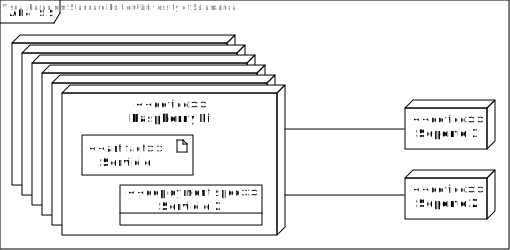
\includegraphics[width=0.8\textwidth]{Chapter4/Figures/Análisis-Componentes}
	\caption[Análisis de componentes]{Análisis de componentes del sistema}
	\label{analisis:componentes}
\end{figure}

\subsection{Interconexión}

Se plantea el uso de cableado físico Ethernet para la comunicación entre los diferentes nodos. Este tipo de conexión es soportada por todos los componentes anteriormente mencionados, y se cuenta con dicho cableado en la infraestructura del centro (ver \ref{dominioproblema:infraestructura}).

\section{Información gestionada por el sistema}

Se plantea un conjunto de requisitos de información gestionados por el sistema pequeño, sin embargo de alta sensibilidad, que el siguiente conjunto de datos.

\subsection{Credenciales de usuario}

Claves de acceso al sistema. Generalmente estas se componen de un par usuario-contraseña. Sin embargo, también se contemplan sistemas alternativos, como la autenticación de en clave pública. La manipulación de la identidad del usuario también es un aspecto clave del sistema.

\subsection{Archivos personales}

Junto a las claves de usuario es necesario gestionar los diferentes ficheros de trabajo que los usuarios manipulen y almacenen en el sistema. Esto implica proporcionar los diferentes mecanismos de acceso a dichos datos y un mecanismo de privilegios (lectura, escritura, ejecución) para impedir la manipulación de forma no deseada de los mismos.

\subsection{Ficheros de configuración e información del sistema}

Diversos componentes del sistema utilizan mecanismos de cifrado cuyas claves no deben ser conocidas por ninguna entidad mas que el administrador del sistema. Los ficheros de configuración del sistema y de las diversas aplicaciones a construir no deben ser modificables por usuarios no autorizados, pues definen aspectos del comportamiento del sistema que pueden comprometer la integridad del mismo si son modificados con fines perniciosos.

\subsection{Registros}

Diversos registros del comportamiento del sistema y de las operaciones realizadas en el mismo serán almacenados en el sistema para su posterior análisis. Dichos ficheros pueden incluir información sensible, como datos de usuarios, por lo que el acceso a los mismos deberá estar restringido.

\subsection{Información de estado}

Si bien la mayor parte de la información se describe en ficheros de carácter permanente, una parte de la información de importancia en el sistema es generada y gestionada por las propias aplicaciones sin almacenar la misma en ningún tipo de soporte permanente. La volatilidad de la información hace que la versatilidad de la misma sea mayor, sin embargo, será necesario contar con una serie de mecanismos que preserven la información frente a circunstancias como recargas de información, reinicios. La manipulación de este tipo de información (actualizaciones, consulta, modificación) presenta una serie de aspectos diferentes a los propios de las estructuras de datos tradicionales.

\subsection{Equipo de soporte}

Como equipos de soporte se plantea el uso del almacenamiento presente en los nodos principales, utilizando, en caso de que sea conveniente, algún nodo secundario como almacén de información.

\section{Identificación de transacciones}

Se plantea el siguiente flujo de transacciones por unidad de tiempo, basado en las estadísticas del sistema (ver \ref{dominio:estadisticast}). La frecuencia de estas operaciones se debe determinar en fases posteriores según estos datos.

\begin{itemize}
\item Operaciones de usuario
\subitem Autenticación contra el sistema.
\subitem Proceso de ficheros.
\subitem Generación de trabajos a realizar por el sistema.
\subitem Realización de pruebas de algoritmos y despliegues.
\item Operaciones de administración.
\subitem Actualizaciones del sistema.
\subitem Operaciones rutinarias de mantenimiento.
\subitem Acceso y análisis de registros.
\end{itemize}

\section{Evolución del sistema}

En caso de proporcionar una solución exitosa para el conjunto de problemas a resolver por el sistema, es esperable un incremento en el número de componentes principales con el fin de aumentar su capacidad de cómputo. Por ello, la escalabilidad del sistema debe ser uno de los requisitos fundamentales del mismo.

\section{Adquisición del sistema}

Los aspectos de la adquisición de los diferentes componentes se definen en \ref{adquisicion}

\section{Identificación de usuarios}

\chapter{Diseño}
\lhead{Diseño}

\section{Portada}
\section{Lista de cambios}
\section{Tabla de contenidos}
\section{Lista de figuras}
\section{Lista de tablas}
\section{Introducción}
\section{Ámbito del software}
\section{Diseño de datos}
\section{Diseño arquitectónico}
\section{Diseño de la interfaz}
\section{Diseño procedimental}
\section{Referencia cruzada a los requisitos}
\section{Pruebas}
\section{Entorno tecnológico del sistema}
\section{Plan de desarrollo e implementación}
\section{Glosario}
\section{Apéndices}